\section{Redes Sociales}

\subsection{¿Qué es una red?}

Una red es un conjunto de relaciones. Mas específicamente, una red consiste en un conjunto de objetos (nodos) que están interconectados a través de relaciones (aristas). La red mas simple consiste en 2 nodos, N1 y N2, que están relacionados entre sí (Figura \ref{fig:simple}). Los nodos podrían representar personas, mientras la arista representa la relación que existe entre ellas (N1 y N2 son amigos, por ejemplo).

\begin{figure}[!htb]
  \begin{center}
    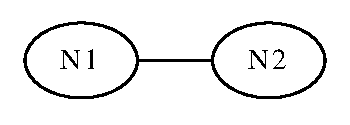
\includegraphics{./imagenes/Red_simple.eps}
    \caption{La red mas simple}
    \label{fig:simple}
  \end{center}
\end{figure}

Las relaciones pueden ser simétricas o asimétricas. Cuando se tiene una relación simétrica se dice que la relación no tiene dirección, es decir, la relación puede leerse en ambos sentidos. En el ejemplo anterior, significaría que N1 es amigo de N2 y que N2 es amigo de N1. Para que una relación se considere asimétrica, la relación debe poder leerse en un único sentido, es decir, la relación tiene una dirección determinada. En la figura \ref{fig:asimetrica} se puede observar un ejemplo de una red asimétrica en donde el nodo (o persona) N1 sigue al nodo N2, pero el nodo N2 no sigue al nodo N1.

\begin{figure}[!htb]
  \begin{center}
    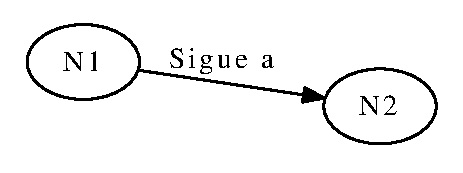
\includegraphics{./imagenes/Red_asimetrica.eps}
    \caption{Ejemplo de una red asimetrica}
    \label{fig:asimetrica}
  \end{center}
\end{figure}

Es posible que exista mas de una relación entre 2 nodos, en ese caso se dice que existe una \textit{relación multiplex}

\subsection{Grado de centralidad}

En todas las redes, sean virtuales o no, existen personas que son mas ``importantes" que otras, más \textbf{populares}. Estas celebridades representan una parte muy pequeña de la red, pero debido a su gran influencia siempre es bueno identificarlos. Para esto se utiliza el \textbf{grado de centralidad}.

El grado de un nodo es la cantidad de conexiones que posee. En una red social, esto se representa por medio de las relaciones que cada nodo tenga, y ya que el significado de la relación varia en función de cada red, es necesario entender que significan las posibles relaciones existentes en una red para hacer el análisis correspondiente. Por ejemplo, en una red como Twitter en donde las relaciones son unidireccionales, puede existir un nodo con un grado de salida muy alto, esto es una persona que sigue a muchas otras. Aunque esta persona tenga un grado de centralidad muy alto, no representa una celebridad, sin embargo, un nodo que tenga un grado de entrada muy alto, que es seguido por muchas personas, si representa una persona que es muy popular en esta red.

\begin{figure}[!htb]
  \begin{center}
    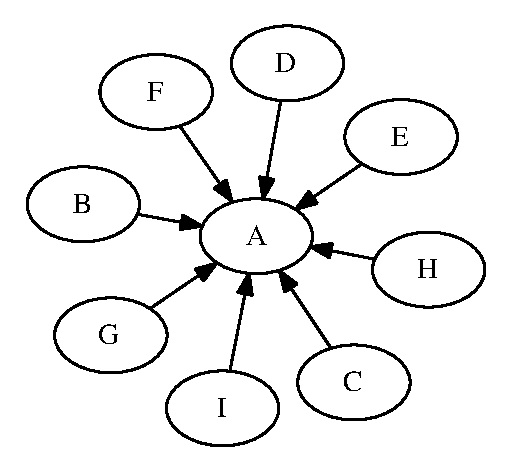
\includegraphics{./imagenes/red_estrella.eps}
    \caption{Red de estrella}
    \label{fig:red_estrella}
  \end{center}
\end{figure}

En la figura \ref{fig:red_estrella} se puede ver un caso en el que el nodo A es una clara celebridad de la red. Este tipo de configuración, llamada red de estrella, es muy poco común en la vida real, pero sirve de ayuda visual para entender a simple vista el concepto de centralidad.

\subsection{Grado de cercanía}

A menudo se puede ver que personas que no tienen mayor influencia aparente en una red son capaces de difundir un mensaje en una gran parte de la red. Esto se debe a que tienen buenas conexiones en la red que les permiten llegar a mas personas, sin que ellos en si sean ``importantes" en la red. Para medir que tan bien o mal posicionado esta un nodo en la red se utiliza el \textbf{grado de cercanía}. Este calculo es bastante caro computacionalmente ya que conlleva una gran cantidad de cálculos.

Los pasos para calcular el grado de cercanía de los nodos de una red son:

\begin{enumerate}
  \item Calcular la ruta mas corta entre todos los pares de nodos posibles, utilizando el algoritmo de Dijkstra, y almacenar estos valores en una tabla.
  \item Para cada nodo de la red:
  \begin{enumerate}
    \item Calcular la distancia promedio con todos los demás nodos.
    \item Dividir el promedio por la distancia mas alta.
    \item Calcular el inverso del valor anterior.
  \end{enumerate}
  \item normalizar cada valor obtenido para obtener valores en el rango de 0-1.
\end{enumerate}

Los nodos que tengan un valor mas cercano a 1 son los que tienen una distancia promedio menor con los nodos de la red, o los que tienen ``\textit{mejores contactos}".

\subsection{Grado de intermediación}

En las redes sociales, suelen formarse grupos mas pequeños que comparten un interés común. Por ejemplo, es mas probable que dos personas que comparten el gusto por los videojuegos interactúen entre si que dos personas que no lo hagan, sin embargo hay casos en los que una persona comparte gustos con diferentes grupos, ayudando a que esta persona se pueda relacionar de manera efectiva con un grupo mas extenso de personas. Estas personas son conocidas como ``puertas frontera" ya que, gracias a ellos, es posible que dos grupos que no tengan nada en común puedan relacionarse entre sí. La medida que ayuda a identificar estos elementos en una red es el \textbf{grado de intermediación}, y consiste en lo siguiente:

\begin{enumerate}
  \item Calcular la ruta mas corta entre todos los pares de nodos posibles, utilizando el algoritmo de Dijkstra, y almacenar estos valores en una tabla.
  \item Para cada nodo n de la red, contar las veces que el nodo n aparece en la lista de rutas mas cortas,
  \item normalizar cada valor obtenido para obtener valores en el rango de 0-1.
\end{enumerate}

Cabe notar que este algoritmo es bastante lento para redes que son muy grandes.

En la figura \ref{fig:bow_tie} se puede ver un claro ejemplo de este fenómeno. Esta red, conocida como la red corbatín (bow-tie en inglés), muestra como el nodo D se encuentra entre 2 grupos de nodos que, de otra manera, no podrían conectarse.

\begin{figure}[!htb]
  \begin{center}
    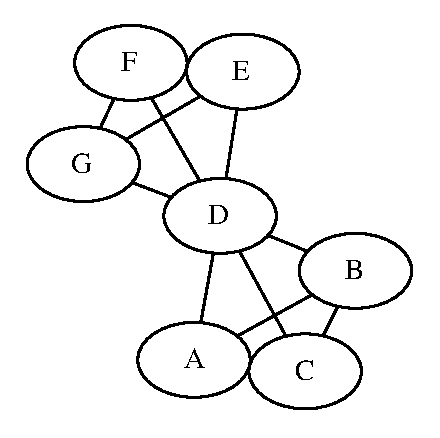
\includegraphics{./imagenes/bow_tie.eps}
    \caption{red corbatín}
    \label{fig:bow_tie}
  \end{center}
\end{figure}

\subsection{Díadas}

Las díadas son la unidad básica de análisis una red social, ya que estas representan la relación entre una y otra persona, esto es, mis amigos, mis seguidores, mis suscriptores, etc. Existen 4 tipos de díadas, representadas en la figura \ref{fig:tipos_diadas}, su uso varia en función del significado de la relación.

\begin{figure}[!htb]
  \begin{center}
      \begin{tabular}{m{3cm}|m{3cm}|m{3cm}|m{3cm}}
        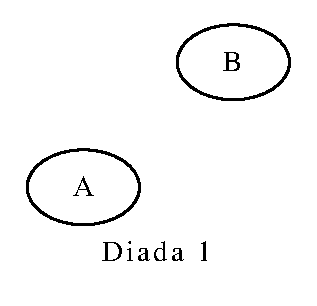
\includegraphics[width=3cm]{./imagenes/diada_1.eps} & 
        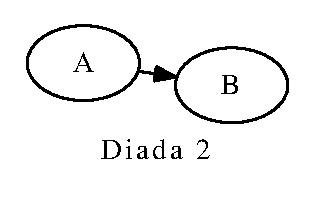
\includegraphics[width=3cm]{./imagenes/diada_2.eps} & 
        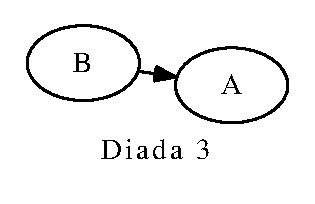
\includegraphics[width=3cm]{./imagenes/diada_3.eps} & 
        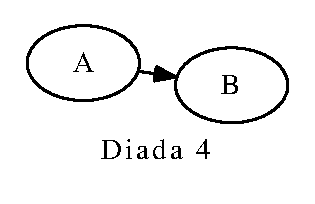
\includegraphics[width=3cm]{./imagenes/diada_4.eps}\\
      \end{tabular}
    \caption{Tipos de diadas asimétricas}
    \label{fig:tipos_diadas}
  \end{center}
\end{figure}

La díada 1 indica que ambos individuos existen en la red, pero todavía no existe ninguna relación entre ellos. Las diadas 2 y 3 muestran una relación unidireccional entre los dos individuos, la única diferencia es el sentido de esa relación. La díada 4, por su parte, es la de mayor interés de las cuatro ya que muestra una relación bidireccional entre los individuos, siendo esta la relación que mayor peso tiene en una red social dado que nos dice que existe un alto grado de reciprocidad en el intercambio de información entra ambos individuos.

\subsection{Tríadas}

Las triadas son básicamente 3 nodos conectados de alguna manera. Al igual que con las diadas, las triadas también pueden ser simétricas o asimétricas, dependiendo estrictamente del contexto en que son utilizadas. Existen 4 tipos de triadas simétricas, ilustradas en la figura \ref{fig:tipos_triadas_simetricas}.

\begin{figure}[!htb]
  \begin{center}
      \begin{tabular}{m{3cm}|m{3cm}|m{3cm}|m{3cm}}
        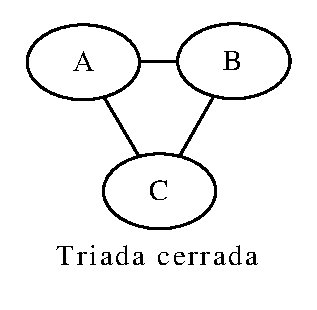
\includegraphics[width=3cm]{./imagenes/triada_simetrica_1.eps} & 
        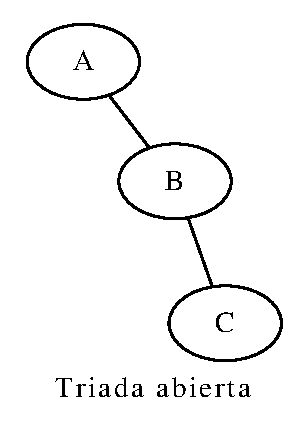
\includegraphics[width=3cm]{./imagenes/triada_simetrica_2.eps} & 
        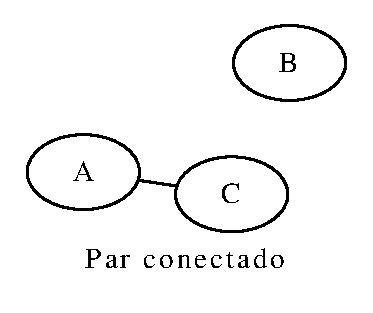
\includegraphics[width=3cm]{./imagenes/triada_simetrica_3.eps} & 
        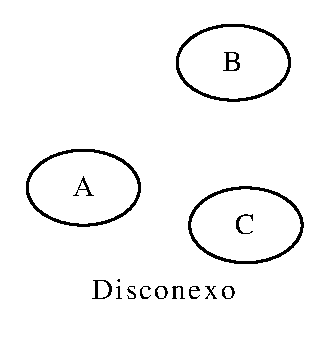
\includegraphics[width=3cm]{./imagenes/triada_simetrica_4.eps}\\
      \end{tabular}
    \caption{Tipos de triadas simétricas}
    \label{fig:tipos_triadas_simetricas}
  \end{center}
\end{figure}

Por otra parte, existen 16 tipos de triadas asimétricas, numeradas del 1-16. Su uso es mas frecuente ya que de ellas se puede hacer un análisis mas complejo en comparación a las díadas. Cada una de estas triadas recibe un nombre especifico para facilitar su identificación, a continuación se explica como debe leerse ese nombre:

\begin{itemize}
  \item El primer numero representa la cantidad de vértices bidireccionales
  \item El segundo numero representa la cantidad de vértices simples
  \item El tercer numero representa la cantidad de vértices inexistentes
  \item Si una triada se repite, se utiliza una letra extra para determinar que variante es:
  \begin{itemize}
    \item U - Arriba (Up)
    \item D - Abajo (Down)
    \item C - Circulo (Circle)
    \item T - Transitiva (Transitive)
  \end{itemize}
\end{itemize}

En la figura \ref{fig:tipos_triadas_asimetricas} se muestran todas las triadas posibles con su respectivo código asociado.

\begin{figure}[!htb]
  \begin{center}
      \begin{tabular}{m{1.3cm}|m{1.3cm}|m{1.3cm}|m{1.3cm}|m{1.3cm}|m{1.3cm}|m{1.3cm}|m{1.3cm}}
        \includegraphics[width=1.3cm]{./imagenes/triada_003.eps} & 
        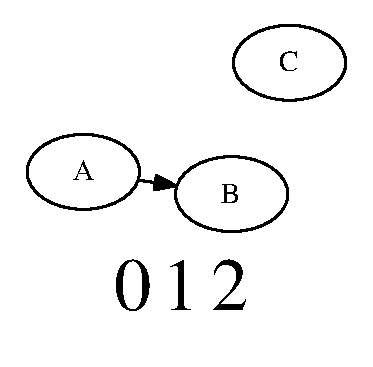
\includegraphics[width=1.3cm]{./imagenes/triada_012.eps} & 
        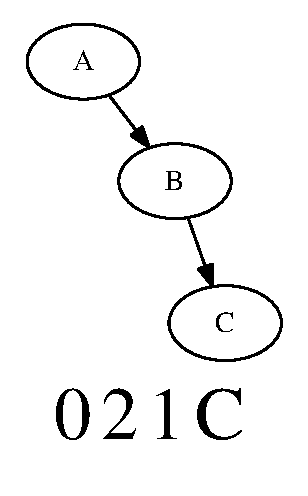
\includegraphics[width=1.3cm]{./imagenes/triada_021C.eps} & 
        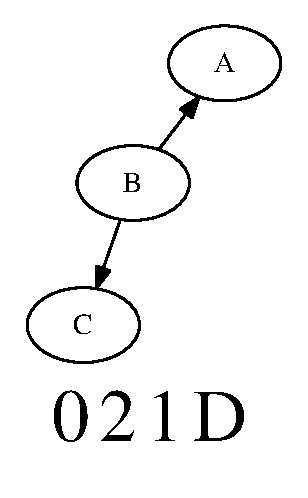
\includegraphics[width=1.3cm]{./imagenes/triada_021D.eps} & 
        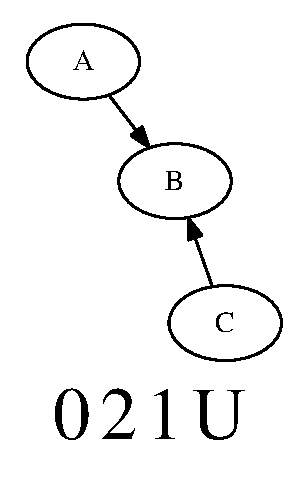
\includegraphics[width=1.3cm]{./imagenes/triada_021U.eps} & 
        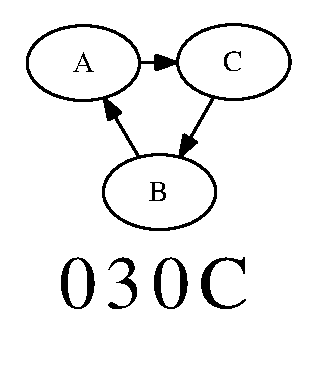
\includegraphics[width=1.3cm]{./imagenes/triada_030C.eps} & 
        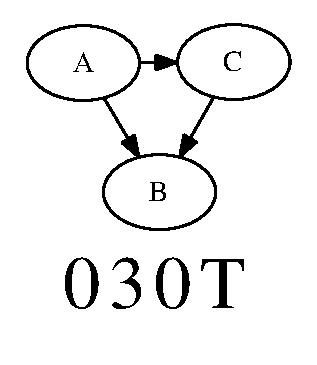
\includegraphics[width=1.3cm]{./imagenes/triada_030T.eps} & 
        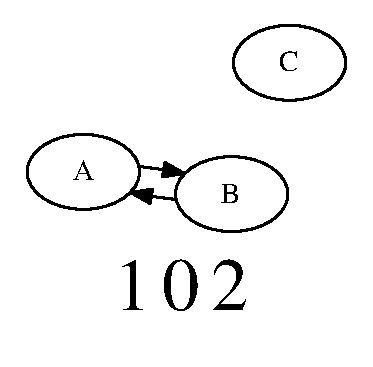
\includegraphics[width=1.3cm]{./imagenes/triada_102.eps}\\ \hline
        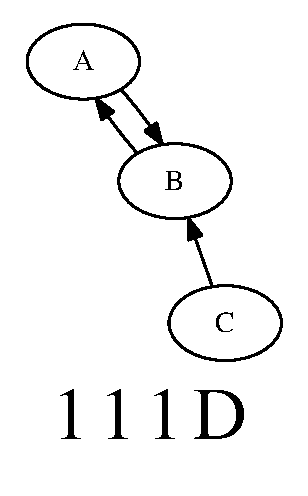
\includegraphics[width=1.3cm]{./imagenes/triada_111D.eps} & 
        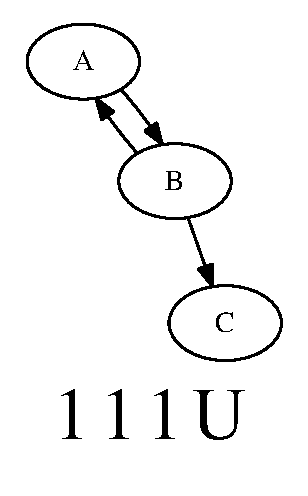
\includegraphics[width=1.3cm]{./imagenes/triada_111U.eps} & 
        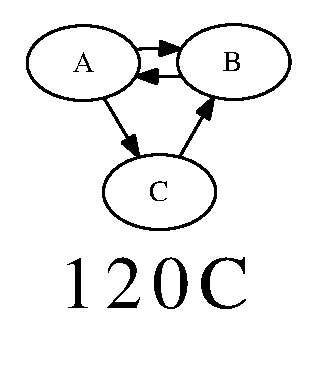
\includegraphics[width=1.3cm]{./imagenes/triada_120C.eps} & 
        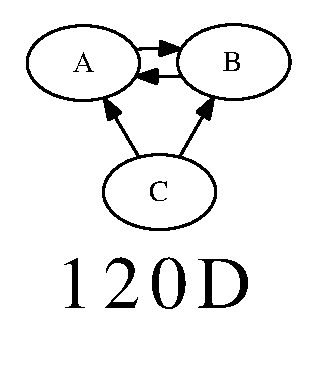
\includegraphics[width=1.3cm]{./imagenes/triada_120D.eps} & 
        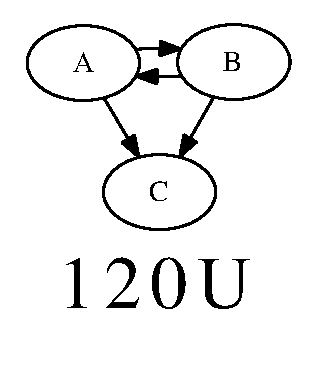
\includegraphics[width=1.3cm]{./imagenes/triada_120U.eps} & 
        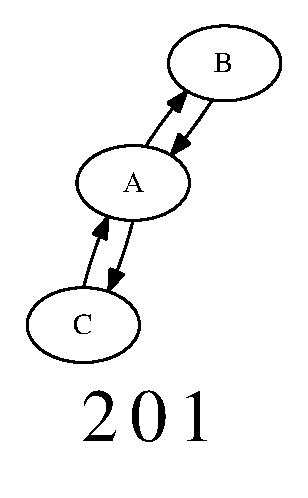
\includegraphics[width=1.3cm]{./imagenes/triada_201.eps} & 
        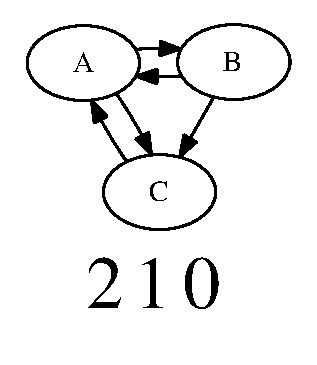
\includegraphics[width=1.3cm]{./imagenes/triada_210.eps} & 
        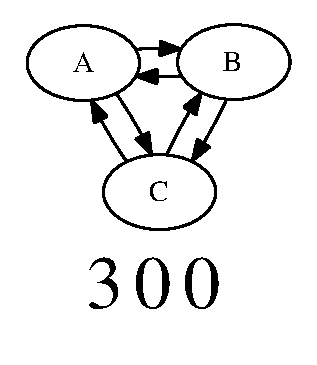
\includegraphics[width=1.3cm]{./imagenes/triada_300.eps}\\
      \end{tabular}
    \caption{Tipos de triadas asimétricas}
    \label{fig:tipos_triadas_asimetricas}
  \end{center}
\end{figure}

Gracias a esta discriminación topológica, se puede hacer un análisis mas completo de una red. Este análisis recibe el nombre de \textbf{\textit{Análisis Triadico}}.

\subsection{Análisis Triadico}

Este proceso, que también recibe el nombre de \textbf{Censo Triadico}, consiste en contar la ocurrencia de cada uno de los tipos de triada para cada nodo, y de esa forma determinar el rol que desempeña este nodo en la red. Por ejemplo, un nodo que presente en mayoría triadas del tipo 4, 7 y 11 es un nodo que \textbf{genera contenido}, mientras que si la mayoría de sus triadas son del tipo 5 y/o 10, es un nodo que recibe o \textbf{consume contenidos}.

Adicionalmente se puede hacer el mismo análisis a la red en general, para tener un punto de vista global de la red. En la figura \ref{fig:red_krackhardt} se puede ver una de las redes mas utilizadas en la teoría de redes sociales, la red de Krackhardt-kite. En esta red se pueden ver muchas características de una red social, facilitando el estudio de las mismas. Al hacer el censo a esta red, nos damos cuenta que presenta una gran cantidad de nodos tipo 201, que representan un agujero estructural, y nodos tipo 300, que representan triadas cerradas, esto nos indica que en esta red existen zonas que tienen una gran concentración de nodos interconectados, mientras hay zonas que no se encuentran muy pobladas. Todo esto se puede ver a simple vista en esta red, pero para redes mas grandes puede que represente un problema mayor.

\begin{figure}[!htb]
  \begin{center}
    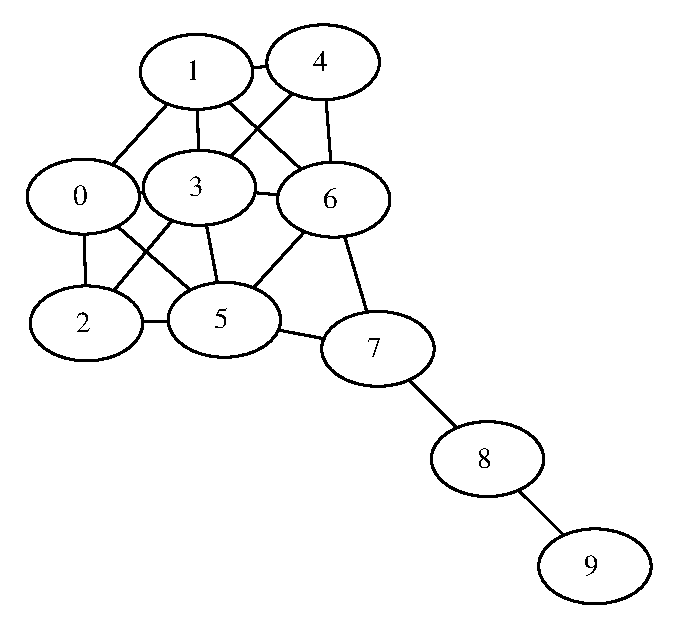
\includegraphics[width=8cm]{./imagenes/red_krackhardt_kite.eps}
    \caption{Red social de Krackhardt kite}
    \label{fig:red_krackhardt}
  \end{center}
\end{figure}

\subsection{Pandillas}
